\chapter{High Level Design Description}
\label{high_level}
This chapter gives an overview of the high level design. It includes a functional block diagram of the system, which partitions the design of the system into blocks, and depicts the interactions between the blocks. The diagram is shown in figure \ref{fig:func_block_diagram}:

\begin{figure}[H]
\centering
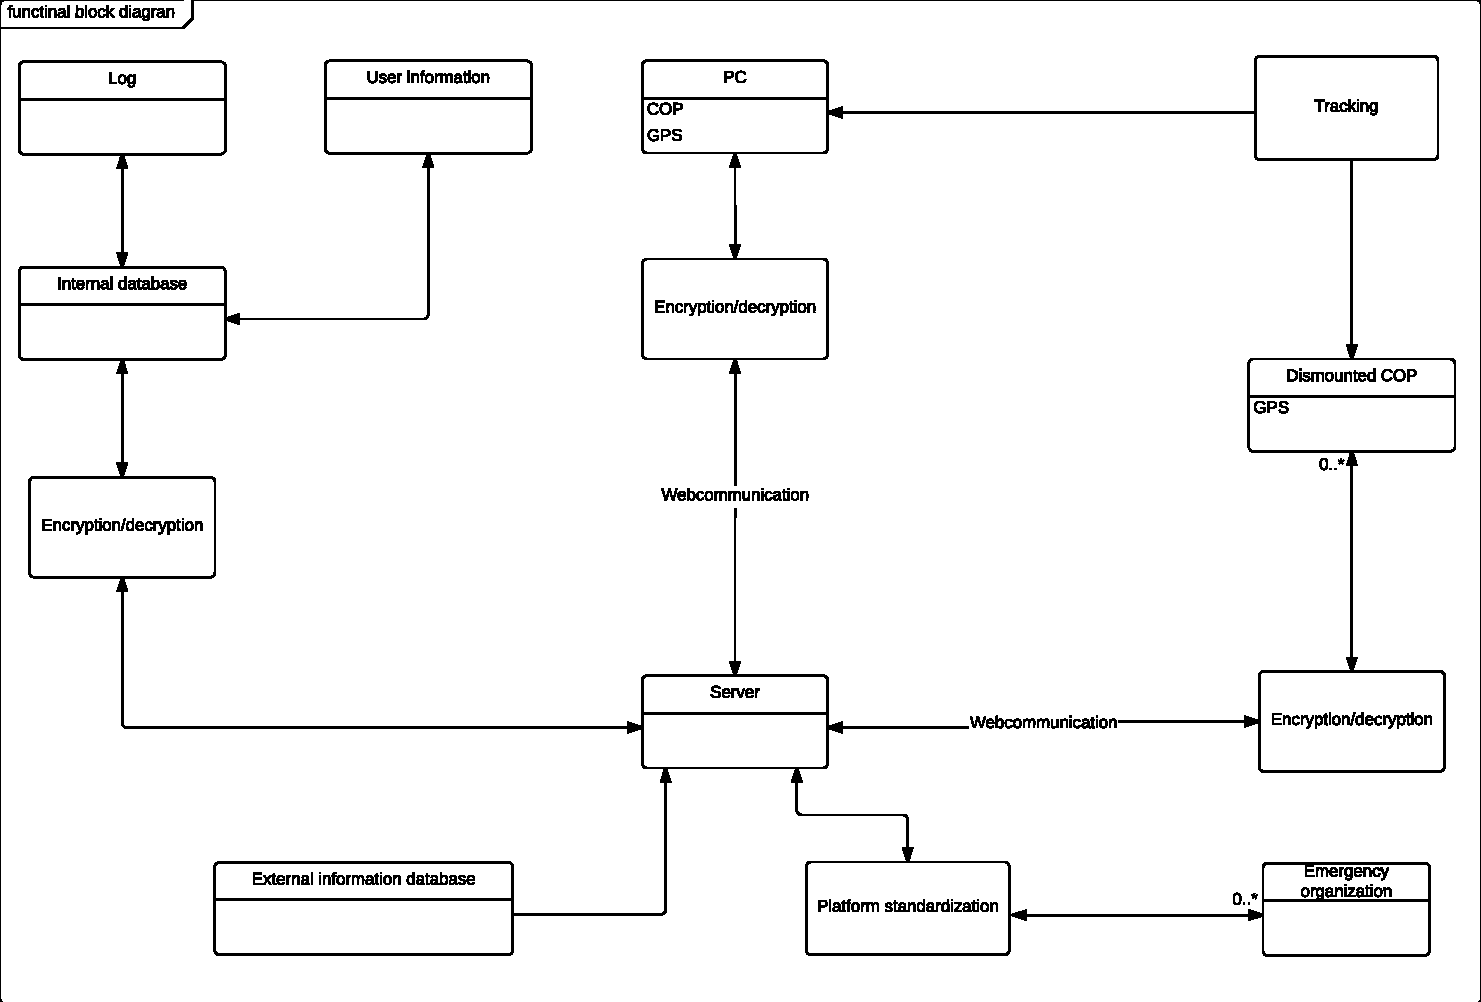
\includegraphics[width=0.95\textwidth]
{billeder/functional_block_diagram.pdf}
\caption{Functional block diagram of the system.}
\label{fig:func_block_diagram}
\end{figure}

The diagram consists of system-blocks and function-blocks. The blocks are depicted as two-compartment blocks with the name of the block in the first compartment, and sub parts in the second compartment. The functions are blocks with a single compartment, containing the name of the function. The system-blocks are actual parts of the system, while the function-blocks are functions and actions that are carried out in the system. The data flow between the blocks are depicted with arrows, whose direction dictates the direction of the data flow. 

\subsubsection{Block description}
In this section a short description of each system- and function-block is given.

\textbf{System-blocks}
\begin{enumerate}
\item[•] \textbf{PC:} This block constitutes the machine in the head quarter (HQ) on which the COP-software will be executed. It also has a GPS, so that the location of the HQ is always known. The PC is to be connected to the internet, in order to be able to communicate with the rest of the system.
\item[•] \textbf{Server:} The server will facilitate communication between the other blocks. In addition, it will store user information along with logs locally in an internal database.
\item[•] \textbf{Log:} The log will contain log entries with information about previous events.
\item[•] \textbf{User information:} 
\end{enumerate}

\textbf{Function-blocks}
\begin{enumerate}
\item[•] \textbf{Encryption/decryption:} 
\end{enumerate}